\chapter{Design di dettaglio}

In questo capitolo sono analizzate nel dettaglio le scelte effettuate dal team per la parte di Design del sistema e della sua realizzazione.

\section{Organizzazione del Codice}
La suddivisione del codice rispecchia il Design Architetturale generale descritto in precedenza ed \`e stato realizzato come in Figura \ref{fig:SudCod}:

\begin{figure}[ht]
\centering
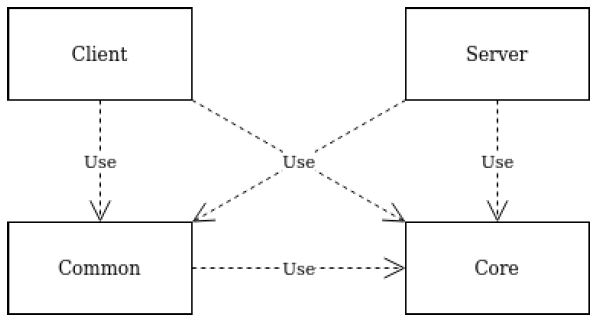
\includegraphics[width=12cm, height=6cm]{img/OrganizationCode.jpg}
\caption{Suddivisione del Codice}
\label{fig:SudCod}
\end{figure}

Sono stati creati 4 moduli principali:
\begin{itemize}
    \item \textbf{Client}: Il Client contiene tutta la parte relativa alle interfacce utente, la comunicazione con il Server e gli aggiornamenti dello stato della partita;
    \item \textbf{Core}: Questo modulo comprende tutte le entit\`a che permettono la realizzazione del gioco e tutti i controlli che rendono possibile il proseguimento di una partita. Questo modulo \`e indipendente dal resto;
    \item \textbf{Common}: In questo modulo \`e presente il codice in comune per le parti di Client e Server. In particolare definisce i messaggi utilizzati per scambiare le informazioni;
    \item \textbf{Server}: Il Server contiene tutta la logica della gestione delle lobby e della varie partite in corso;
\end{itemize}

\section{Core}
Il Core si occupa della modellazione di tutte le entit\`a del gioco Among Us, come i personaggi, le possibili abilit\`a (\textit{Kill} e \textit{Sabotage}) e le funzionalit\`a base del gioco (\textit{Movement}, \textit{Report} e \textit{Emergency}). Serve, quindi, per permettere agli altri moduli del progetto di interagire con le entit\`a. Queste funzioni implementano tutte le azioni che un giocatore potr\`a svolgere nel gioco reale.

\subsection{Drawable}
\begin{figure}[ht]
\centering
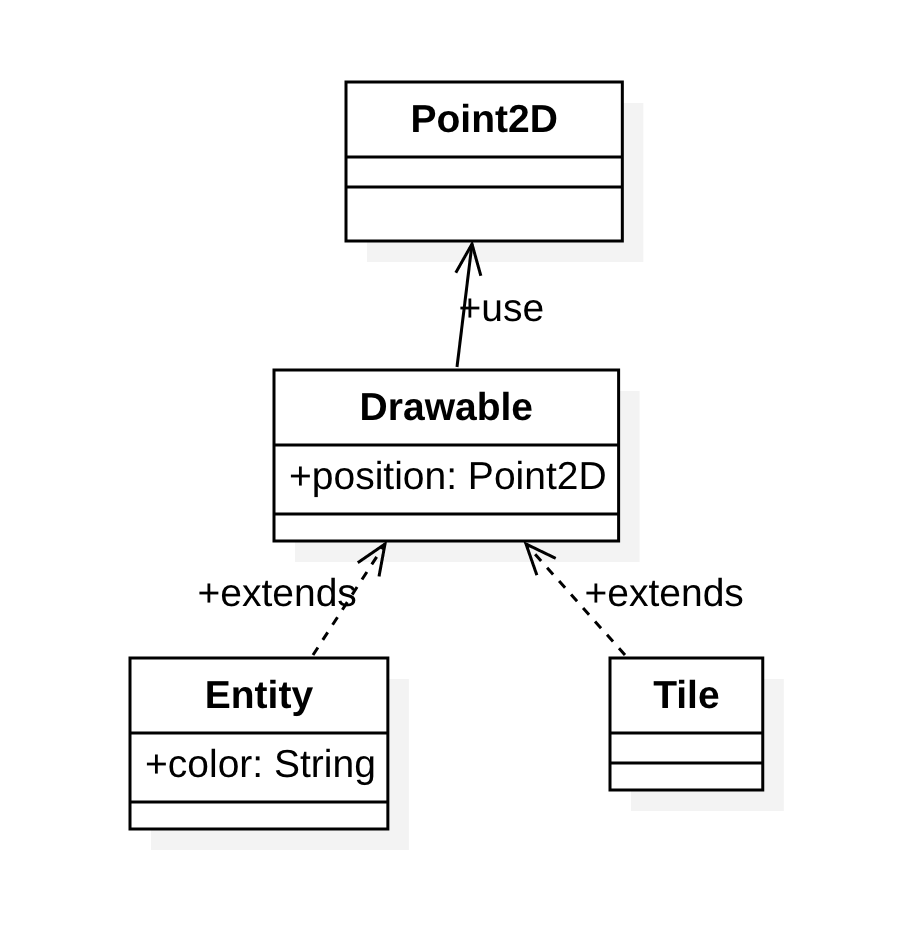
\includegraphics[width=7cm, height=7.5cm]{img/drawable.png}
\caption{Class Diagram che rappresenta Drawable}
\label{fig:ClasDiagRaprDraw}
\end{figure}

Come si può vedere dalla Figura \ref{fig:ClasDiagRaprDraw} le due entit\`a principali del gioco sono \textit{Tile} ed \textit{Entity}. Entrambe estendono da \textit{Drawable}, la quale rappresenta tutti gli oggetti disegnabili all'interno della mappa di gioco in una determinata posizione. 
\subsection{Tile}
\begin{figure}[ht]
\centering
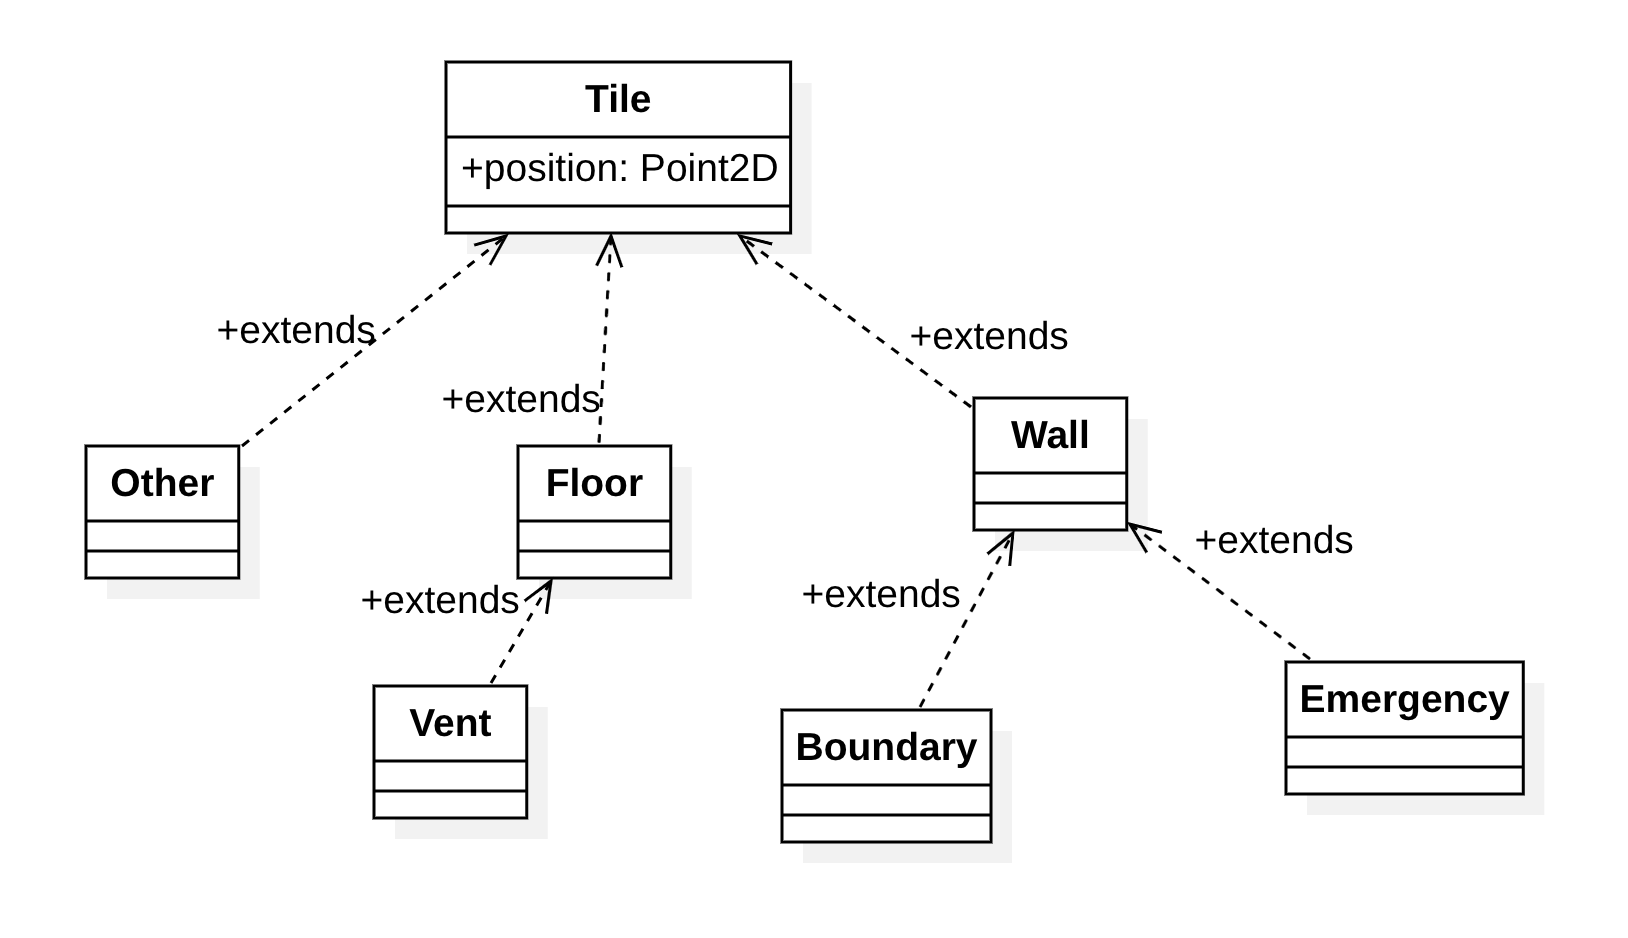
\includegraphics[width=\textwidth, scale=0.44]{img/tile.png}
\caption{Class Diagram che rappresenta Tile}
\label{fig:ClasDiagRaprTile}
\end{figure}
Tutti gli elementi statici che compongono la mappa estendono da \textit{Tile} come mostrato nella Figura \ref{fig:ClasDiagRaprTile} e sono i seguenti:
\begin{itemize}
    \item \textit{Wall}: Rappresenta i muri della mappa di gioco, questi non potranno essere attraversati dai giocatori vivi ma solamente da quelli morti;
    \item \textit{Floor}: Rappresenta il pavimento della mappa di gioco, sopra il quale tutti i giocatori potranno muoversi;
    \item \textit{Vent}: Rappresenta una cella particolare del pavimento e permette agli Impostori di spostarsi rapidamente sulla mappa in quanto ogni Vent risulta collegata ad una sua "gemella";
    \item \textit{Boundary}: Rappresenta il confine invalicabile della mappa oltre il quale nessun giocatore vivo o morto potr\`a andare;
    \item \textit{Other}: Rappresenta gli spazi vuoti all'interno della mappa ai quali solo i fantasmi potranno accedere; 
    \item \textit{Emergency}: Rappresenta un particolare tipo di muro con il quale tutti i giocatori vivi potranno interagire una volta per partita;
\end{itemize}

\subsection{Entity}

\begin{figure}[ht]
\centering
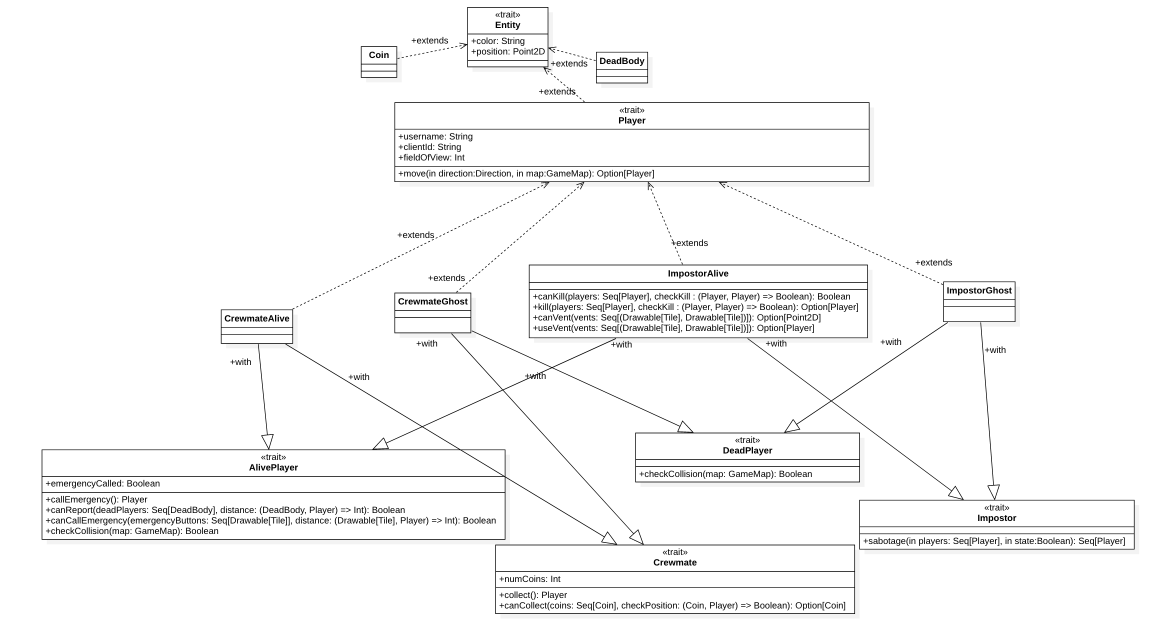
\includegraphics[width=13cm, height=11cm]{doc/report/img/ClassCore.png}
\caption{Class Diagram che rappresenta Entity}
\label{fig:ClasDiagRaprEnt}
\end{figure}

Gli elementi dinamici che compongono la mappa estendono da \textit{Entity} sono mostrati in Figura \ref{fig:ClasDiagRaprEnt}, ed a differenza della \textit{Tile} possiedono anche un colore relativo all'oggetto rappresentato. Tutti gli oggetti di questo tipo sono visualizzati sopra le \textit{Tile} e sono i seguenti:
\begin{itemize}
    \item \textit{DeadBody}: Rappresenta il cadavere di un giocatore morto a causa dell'Impostore;
    \item \textit{Coin}: Rappresenta tutti i collezionabili che possono essere raccolti dai Crewmate vivi e/o morti;
    \item \textit{Player}: Rappresenta il giocatore base del gioco;
\end{itemize}

\subsubsection{Player}
Per quanto riguarda il Trait \textit{Player} esso modella i tipi di giocatore presenti all'interno di una partita. Oltre al colore ed alla posizione ereditati da \textit{Entity} aggiunge:
\begin{itemize}
    \item \textit{Username}: Campo che rappresenta il nome del giocatore che verr\`a renderizzato sopra al personaggio;
    \item \textit{Client ID}: Campo univoco utilizzato per distinguere i vari giocatori;
    \item \textit{Field Of View}: Campo di visuale variabile in base al tipo del giocatore;
    \item \textit{Move}: Metodo che gestisce il movimento del giocatore all'interno della mappa;
\end{itemize}
I giocatori possono essere delle seguenti tipologie:
\begin{itemize}
    \item \textit{Crewmate Alive}: Rappresenta il giocatore buono che ha lo scopo di raccogliere tutte le \textit{Coin} presenti nella mappa di gioco, pu\`o inoltre, in caso di ritrovamento di un cadavere, segnalarlo agli altri giocatori tramite la funzione \textit{Report}. Ulteriormente, una volta per partita, pu\`o effettuare una chiamata di emergenza ed attivare la fase di votazione tramite l'\textit{Emergency Button};
    \item \textit{Impostor Alive}: Rappresenta il giocatore cattivo che ha lo scopo di uccidere tutti i giocatori buoni della partita senza farsi scoprire e/o essere eliminato durante le varie fasi del gioco. Inoltre, pu\`o attivare un sabotaggio che gli permette di confondere i giocatori \textit{Crewmate} ed utilizzare le \textit{Vent} del gioco per spostarsi rapidamente da un punto all'altro della mappa;
    \item \textit{Crewmate Ghost}: Rappresenta il giocatore buono ucciso durante una partita. Questo tipo di giocatore pu\`o solamente terminare la raccolta delle proprie Coin per portare la sua squadra alla vittoria;
    \item \textit{Impostor Ghost}: Rappresenta il giocatore cattivo morto dopo una fase di votazione e la sua unica funzione \`e quella di aiutare i suoi compagni vivi utilizzando in modo strategico i sabotaggi;
\end{itemize}

Al fine di rendere modulare l'acquisizione di diversi comportamenti attraverso l'algoritmo di linearizzazione predisposto da scala, per la modellazione degli aspetti strutturali dei \textit{Player}, si \`e sfruttato il meccanismo dei \textbf{Self-Type}.\\
Tale pattern di programmazione \`e un modo per dichiarare che un \textit{trait} deve essere combinato tramite \textit{mixin} in un altro \textit{trait}, pur non estendendolo direttamente. Tramite questa tecnica è possibile fare \textit{dependency injection} dichiarando esplicitamente nel \textit{trait} le dipendenze di cui un componente necessita. Uno dei vantaggi della separazione del comportamento dalla struttura \`e quello della riusabilit\`a dei concetti e quindi del codice. Mettendo assieme strutture e comportamenti \`e possibile combinarli e riutilizzarli per estensioni e implementazioni future.\\
Una volta definiti un set di propriet\`a ed i \textit{self-type} corrispondenti, la definizione della componente strutturale dei \textit{Player} si riduce ad un'attivit\`a di composizione di moduli elementari. Ci\`o porta ad una struttura composta da pi\`u livelli di componenti, alcuni dei quali condivisi da pi\`u \textit{Player}. Questo approccio rende riutilizzabili in futuro le astrazioni gi\`a definite permettendo di combinare i diversi comportamenti con flessibilit\`a.\\
Focalizzando l'attenzione sull'implementazione mostrata nella Figura \ref{fig:ClasDiagRaprEnt} la classe \textit{CrewmateAlive} estende dal \textit{trait Player} che ne definisce la struttura. Il comportamento \`e invece definito nei \textit{trait Crewmate} e \textit{AlivePlayer}. D'altra parte \`e possibile notare che anche \textit{ImpostorGhost} mantiene la struttura derivata dal \textit{Player}, ma il suo comportamento è descritto in \textit{Impostor} e in \textit{DeadPlayer}.\\
Per gestire il movimento dei diversi tipi di giocatori si \`e fatto uso del meccanismo delle \textbf{type class}. Il metodo \textit{movePlayer} \`e stato reso generico e quindi utilizzabile da qualsiasi tipo di giocatore. Successivamente, in base al tipo di giocatore, viene fornita in maniera implicita una differente strategia di movimento. Inoltre, per ridurre il \textit{boilerplate code} riguardante l'aggiornamento della posizione del giocatore, \`e stato utilizzato il pattern \textbf{Pimp my library} sulla classe \textit{Point2D}.\\
\textit{Pimp My Library} consente di estendere un tipo aggiungendovi metodi senza l'utilizzo dell'ereditariet\`a. Utilizzando questo Pattern si pu\`o aggiungere un metodo senza bisogno di estenderlo, attraverso conversioni implicite. Questa soluzione ha permesso di alzare il livello di astrazione del codice permettendo di ignorare i dettagli relativi alla costruzione della soluzione implementativa.

\subsection{Prolog}
Successivamente allo sviluppo delle funzionalit\`a del core effettuato sfruttando il paradigma funzionale, tutto il team ha prodotto alcune di queste utilizzando la programmazione logica.
L’integrazione \`e stata realizzata grazie alla libreria \textbf{TuProlog}.\\
In particolare \`e stata implementata la logica del movimento dei vari giocatori sia vivi che morti controllando tutte le possibili collisioni.\\
Oltre a questo sono state implementate alcune funzioni utili al calcolo della distanza fra due punti della mappa e fra un punto e lista di punti restituendo solo i punti della lista  con distanza minore di un particolare input specificato.\\
Queste implementazioni possono tornare utili nel caso in cui \`e necessario controllare se l’impostore pu\`o effettuare una \textit{kill}, oppure se un giocatore qualsiasi può effettuare l’operazione di report.\\
Tutte queste implementazioni non sono state richiamate nello sviluppo del gioco ma solamente testate nella classe \textit{PrologTest}.\\
La teoria Prolog brevemente descritta \`e presente nel file \textit{core/resources/theory.pl}.

\section{Common}
Il common \`e stato impiegato per raggruppare tutta la parte di codice in comune tra il modulo del Server e quello del Client. In particolare sono stati inseriti i vari messaggi che entrambi i moduli dovranno scambiarsi, qualche metodo per fare logging e le costanti necessarie per il corretto funzionamento della connessione Client-Server.

\section{Server}
Questo modulo rende possibile il corretto svolgimento del gioco. Ogni sessione dei vari giocatori \`e possibile dividerla in due fasi:
\begin{itemize}
    \item \textbf{Lobby}: Avviata l'applicazione, l'utente pu\`o connettersi al Server inviandogli i dati necessari per creare o entrare in una partita. Una volta connessi si viene inseriti in una lobby e si deve attendere finch\`e non si raggiunge un numero sufficiente di partecipanti per iniziare la partita. Al raggiungimento del numero minimo di giocatori (impostato in fase di avvio della partita), tutti i player sono rimossi e viene avviato il gioco;
    \item \textbf{Game}: Si occupa della gestione della partita. Nella fase di inizializzazione il Server comunica ai Client che \`e stata trovata una partita. Prima che il gioco cominci il server genera lo stato iniziale della partita e lo comunica ai giocatori. Successivamente si occupa di ritrasmettere i vari aggiornamenti di stato da parte di ciascun giocatore, andando a verificare se vi \`e presente una condizione di vittoria. Se una di queste condizioni \`e verificata, il Server notifica a tutti i giocatori il termine della partita, altrimenti invia un messaggio di aggiornamento;
\end{itemize}

\subsection{Lobby}
\begin{figure}[ht]
\centering
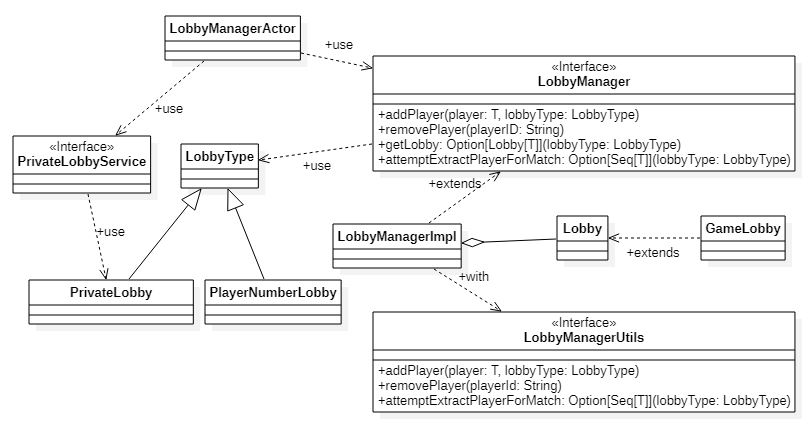
\includegraphics[width=\textwidth, scale=0.44]{img/LobbyUML.jpg}
\caption{Class Diagram che rappresenta LobbyManagerActor}
\label{fig:ClasDiagRaprLobbyManagerActor}
\end{figure}

Per quanto riguarda la parte delle Lobby rappresentato nella Figura \ref{fig:ClasDiagRaprLobbyManagerActor}, \`e stato realizzato l'attore LobbyManagerActor che si occupa della gestione della fase iniziale del gioco. Esso \`e stato creato estendendo il \textit{Trait Actor} di Akka rendendo possibile la ricezione di messaggi provenienti dal modulo Client.\\
Buona parte della logica di questo componente \`e stata spostata fuori in altre strutture dati seguendo il pi\`u possibile il principio di \textit{Separation of Concerns}.\\
La struttura base della Lobby \`e rappresentata da una lista di giocatori con le stesse impostazioni di gioco e con il medesimo numero di partecipanti. Per il \textit{Trait Lobby} si \`e deciso di implementare il Pattern \textbf{Pimp My Library} implementando la classe \textit{RichLobby} per una pi\`u attenta riorganizzazione della struttura.\\
Il componente \textit{LobbyManager}, invece, \`e il componente che si occupa del mantenimento dei riferimenti a tutte le lobby create durante l'esecuzione del sistema. Esso espone i metodi per rimuovere, estrarre e creare giocatori da una determinata Lobby.\\
Per realizzare tutto ci\`o, \textit{LobbyManager} mantiene una Lobby in corrispondenza di ogni \textit{LobbyType} avente le informazioni sulle sue caratteristiche. Inoltre, si \`e deciso di implementare al suo interno il Pattern \textbf{Self-Type} per rendere modulari i comportamenti della Lobby.

\subsubsection{Modellazione delle Private Lobby}
Le \textit{PrivateLobby} mantengono le medesime caratteristiche di una Lobby normale e, in aggiunta, possiedono un codice univoco per poter essere identificate.
La Classe \textit{PrivateLobbyService} si occupa del supporto alla creazione delle lobby private, generando un ID univoco ad ogni richiesta.

\subsection{Game}
\textit{GameManagerActor} \`e l'attore del server che si occupa della gestione della partita, creato dall'attore \textit{LobbyManagerActor} precedentemente descritto.\\
Questo Attore non mantiene lo stato globale della partita in quanto queste informazioni vengono mantenute all'interno di ciascun Client. Questa scelta \`e stata effettuata per ridurre il numero di messaggi scambiati tra Client-Server e ridurre il carico di lavoro del Server. Ciascun Client quindi prima di notificare il cambiamento del proprio stato esegue una serie di operazioni interne e, solo successivamente, notificher\`a il Server.\\
Lo svantaggio di questa architettura consiste nella possibilit\`a da parte del Client di inviare uno stato fittizio al Server che non avrebbe alcun modo di verificarlo, andando a trasmetterlo a tutti gli altri giocatori.

\subsection{Fault Tolerance}
Per la realizzazione di tutte le componenti citate, si \`e cercato di gestire al meglio tutte le eventuali possibili situazioni di errore che si possono presentare, come ad esempio la disconnessione improvvisa di uno dei Client connessi. Per fare ci\`o si \`e fatto utilizzo delle funzionalit\`a di supervisione e monitoraggio messe a disposizione da parte del Framework Akka.\\
Avendo a disposizione il riferimento dell'attore, \`e stato possibile mettersi in ascolto su un'eventuale evento di terminazione tramite messaggio \textit{Terminated}. Queste funzionalit\`a sono state sfruttate dall'attore Lobby per rimuovere gli utenti disconnessi dalle code.\\
L'attore responsabile delle partite, a fronte della terminazione di uno dei Client, notificher\`a tutti gli altri giocatori dell'avvenuta disconnessione, specificando l'ID del giocatore disconnesso.

\section{Client}
Per quanto riguarda il Client si \`e scelto di utilizzare un'\textbf{Architettura ad Attori} affiancata dal \textbf{Pattern MVC}.\\
Ogni componente ha quindi un proprio attore, il ModelActor \`e responsabile del Model, il \textit{ControllerActor} del Controller ed infine lo \textit{UiActor} per la parte di View.\\
Questa scelta ci ha consentito di ottenere all'interno del Client una buona separazione dei concetti tra le varie classi ed un'efficiente scambio di informazioni tramite i messaggi.\\
All'avvio dell'applicazione, tramite la classe \textit{AppLauncher}, viene richiamato il \textit{Controller}.

\subsection{Controller}
\begin{figure}[ht]
\centering
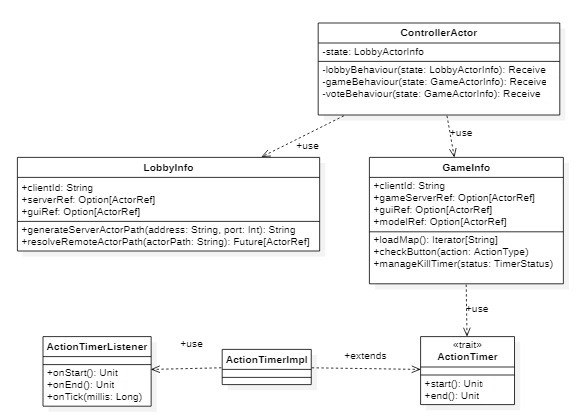
\includegraphics[width=\textwidth, scale=0.44]{doc/report/img/Class-diagram-Controller.jpeg}
\caption{Class Diagram che rappresenta il ControllerActor}
\label{fig:ClasDiagRaprControlAct}
\end{figure}

Il Controller ha il compito di istanziare e far partire il \textit{ControllerActor}, rappresentato nella Figura \ref{fig:ClasDiagRaprControlAct}, il quale deve gestire lo scambio di messaggi interno al Client e la comunicazione con il server.\\
Per gestire al meglio le diverse fasi previste dall'applicazione, si \`e optato per la creazione di diversi comportamenti che possono essere assunti dal \textit{ControllerActor} durante l'esecuzione:
\begin{itemize}
    \item \textbf{Lobby}: In questo comportamento l’attore ha come primo compito quello di stabilire una connessione con il Server. Per fare ci\`o deve andare a reperire l'indirizzo dell'attore del Server dal file di configurazione e generare il suo riferimento attraverso i metodi presenti in \textit{LobbyInfo}. Successivamente si deve occupare della gestione dei messaggi inerenti alla fase di \textit{match making} e della possibile terminazione dell'applicazione da parte dell'utente. Infine, istanzia il \textit{ModelActor} una volta terminata la fase di \textit{match making} modificando poi il suo comportamento in quello di \textit{Game};
    \item \textbf{Game}: Coordina tutto lo svolgimento del gioco aggiornando la View in seguito ad un cambiamento del Model, e viceversa. Essendo l’unico attore in grado di comunicare con il server riceve tramite messaggio tutti i cambi di stato degli altri giocatori notificandoli al Model. Nel caso in cui il proprio giocatore utilizza tramite la View il bottone destinato alla \textit{Kill} o al \textit{Sabotage} avvia un countdown avvalendosi della trait ActionTimer. Diversamente se il giocatore preme \textit{Report} o \textit{Emergency} l'attore cambia il proprio comportamento passando a quello di \textit{Vote};
    \item \textbf{Vote}: Si occupa di quella fase di gioco in cui tutti i giocatori potranno votare un altro giocatore da eliminare. Ulteriormente a ci\`o, gestisce l'invio e la ricezione di eventuali messaggi nella Chat. Finita la fase di votazione ritorna nel comportamento del \textit{Game};
\end{itemize}

\subsection{Model}
\begin{figure}[ht]
\centering
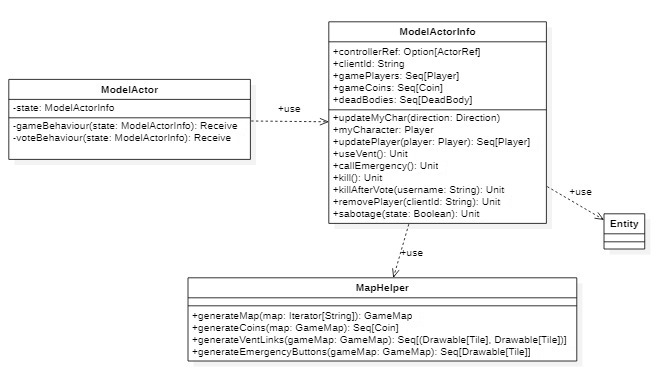
\includegraphics[width=\textwidth, scale=0.44]{doc/report/img/Class-diagram-Model.jpeg}
\caption{Class Diagram che rappresenta il ModelActor}
\label{fig:ClasDiagRaprModelAct}
\end{figure}

Il Model nel Client \`e composto esclusivamente dal \textit{ModelActor} rappresentato nella Figura \ref{fig:ClasDiagRaprModelAct}, da \textit{ModelActorInfo} utile per gestirne lo stato e da \textit{ModelActorMessages} che contiene tutti i tipi di messaggio che \`e possibile ricevere.\\
Il \textit{ModelActor} ha il compito di ricevere notifiche, da parte del \textit{ControllerActor}, riguardanti azioni compiute dall'utente e/o di aggiornamento degli altri giocatori. In seguito alla ricezione di un messaggio di aggiornamento provvede ad aggiornare lo stato del Model ed a notificare a sua volta il \textit{ControllerActor} del cambiamento di stato interno del Model.\\
Per fare ci\`o sono stati ideati due comportamenti:
\begin{itemize}
    \item \textbf{Game}: Si occupa inizialmente della generazione della mappa e delle \textit{Coin} destinate ai \textit{Crewmate} facendo uso dei metodi forniti da \textit{MapHelper}. In particolare questo comportamento gestisce tutta la logica del gioco andando a verificare, utilizzando le funzioni del \textbf{Core}, se le azioni compiute da un giocatore sono valide o meno. Dopodich\`e va ad aggiornare lo stato del \textit{ModelActorInfo}. In seguito verifica se il giocatore ha la possibilit\`a di interagire con i vari elementi della mappa (\textit{Vent}, \textit{Emergency Button}, etc..) oppure con altri giocatori. Infine pu\`o cambiare il suo comportamento in Vote oppure, in caso di abbandono della partita da parte del giocatore, provvede a terminare se stesso;
    \item \textbf{Vote}: Questo comportamento si occupa dell'aggiornamento dei giocatori deceduti durante la fase di votazione, andando a notificare al Controller l'aggiornamento della lista dei giocatori deceduti e far tornare la partita nella fase di gioco;
\end{itemize}

\newpage
\subsection{View}

\begin{figure}[ht]
\centering
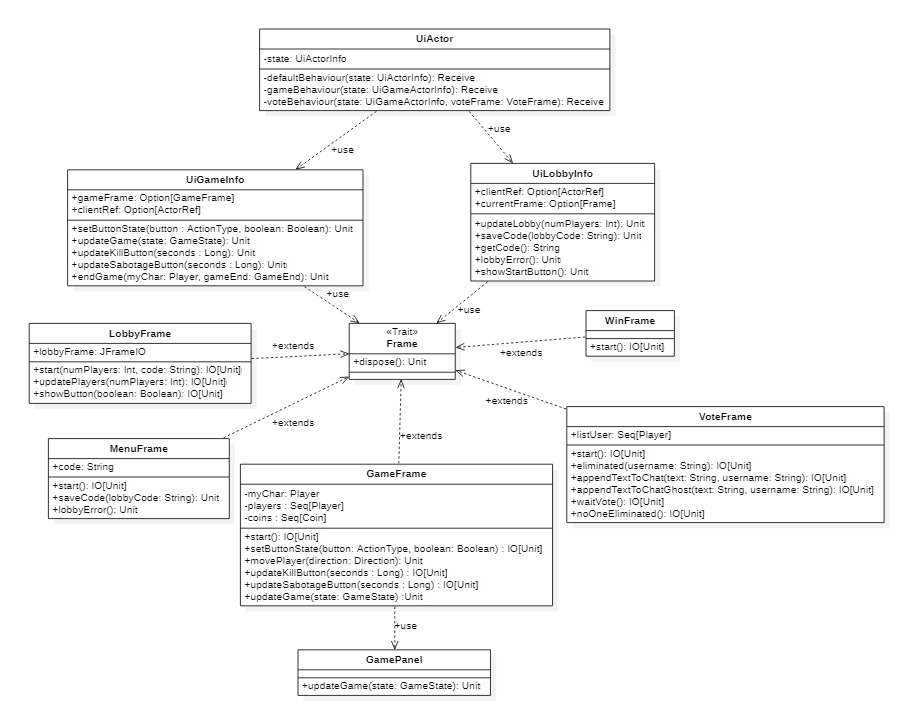
\includegraphics[width=13cm, height=12cm]{doc/report/img/Class-diagram-View.jpeg}
\caption{Class Diagram che rappresenta UiActor}
\label{fig:ClasDiagRaprUiAct}
\end{figure}

In questo componente l'entit\`a attiva \`e un attore chiamato UiActor, rappresentato in Figura \ref{fig:ClasDiagRaprUiAct}, il quale comunica al \textit{ControllerActor} le azioni dell'utente.\\
Inoltre, aggiorna quando opportuno i vari Frame della GUI per mostrando i cambiamenti del Model.\\
L'\textit{UiActor} pu\`o assumere uno dei seguenti comportamenti:
\begin{itemize}
    \item \textbf{Lobby}: In questo comportamento l'\textit{UiActor} è in grado di gestire tutte le operazioni di matchmaking. In dettaglio si occupa della gestione del \textit{MenuFrame} e del \textit{LobbyFrame}.\\
    Comunica con il \textit{ControllerActor} ogni qualvolta l'utente voglia partecipare o creare una Lobby Pubblica o Privata. Visualizza e notifica all'utente l'entrata e l'uscita di giocatori nella Lobby. Inoltre, provvede alla generazione del \textit{GameFrame} una volta raggiunto il numero minimo di partecipanti e cambia il proprio comportamento in quello di \textit{Game};
    \item \textbf{Game}: \`E il comportamento che si occupa di notificare al \textit{ControllerActor} tutte le azioni che il giocatore vuole effettuare. In particolare il giocatore pu\`o muovere il proprio personaggio tramite i comandi sulla tastiera oppure premere uno dei bottoni della GUI presenti nel \textit{GameFrame}. Controlla il risultato del Timer delle azioni dell'impostore notificato dal \textit{ControllerActor}. A seguito di un azione di tipo \textit{Report} o \textit{Emergency} cambia il proprio stato in Vote;
    \item \textbf{Vote}: Questo comportamento gestisce la GUI nella fase in cui l'utente deve esprimere il proprio giudizio selezionando un giocatore da eliminare. Inoltre visualizza gli eventuali messaggi inviati tramite la Chat all'interno del \textit{VoteFrame}. In particolare, scambia alcuni messaggi con il \textit{ControllerActor} relativi alla notifica del voto dei giocatori, la comunicazione del giocatore eliminato, l'invio e la ricezione dei messaggi relativi alla chat. Alla fine della fase di votazione cambia il proprio comportamento in \textit{Game};
\end{itemize}

\subsubsection{Type class}
Degno di nota \`e il modo in cui viene effettuato il rendering delle \textit{Tile} e delle \textit{Entity} per il quale \`e stato utilizzato il meccanismo delle \textit{type class}.\\
Una \textit{Type class} non \`e altro che un gruppo di tipi che soddifano un contratto tipicamente definito in un \textit{trait}.\\
Questo permette di rendere una funzione polimorfica ad-hoc senza modificarne il suo codice. Infatti l'effettiva implementazione \`e definita in maniera implicita a seconda del tipo che richiama quest'ultima.\\
Questo pattern funzionale \`e visibile all'interno del package view.draw.

\subsubsection{Wrapper Monadico di Swing}
Per quanto riguarda lo sviluppo dei Frame presenti nella GUI, si \`e optato di utilizzare il framework \textbf{Cats.IO} per realizzare un \textit{Wrapper} Monadico di \textbf{Swing}. Quest'ultimo permette l'accesso alle API pi\`u comuni dei principali componenti della libreria \textit{Swing}. Ulteriormente, tramite questa implementazione \`e possibile sostituire il tradizionale metodo ad oggetti di chiamate ai metodi con un insieme di funzioni di tipo \textit{IO Monad}. All'interno dei corpi di quest'ultime vi saranno tutte le operazioni necessarie alla realizzazione della GUI. Mentre tutti i side effect avverranno solamente al momento dell'esecuzione della monade. Inoltre, i risultati non saranno memorizzati, il che significa che il sovraccarico di memoria \`e minimo e anche che un singolo effetto pu\`o essere eseguito pi\`u volte in modo referenzialmente trasparente.\\
Un altro vantaggio derivante da questa scelta \`e la possibilità di riutilizzare il package contenente il wrapping monadico in altre applicazioni o di espanderlo con facilit\`a in futuro in quanto risulta completamente indipendente dal resto del gioco.

\newpage
\section{Interazione Client-Server}
\subsubsection{Comunicazione fase Lobby}

\begin{figure}[ht]
\centering
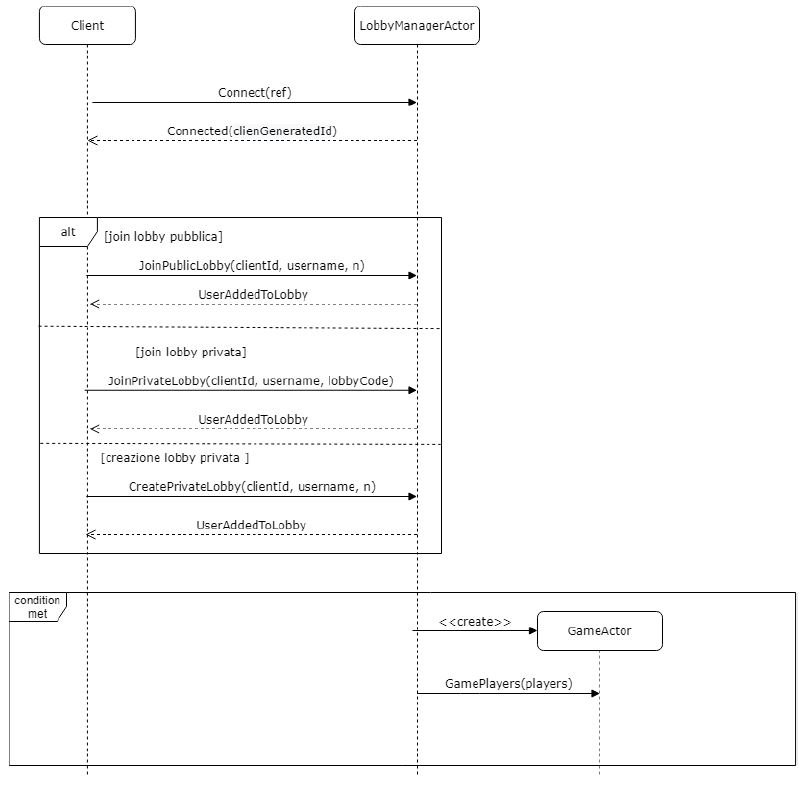
\includegraphics[width=13cm, height=12cm]{img/InteractionWithClient.jpg}
\caption{Sequence Diagram che rappresenta l'interazione con il Client}
\label{fig:ClasDiagRaprInterazClient}
\end{figure}

Per connettere un Client ad una Lobby e poter accedere e/o partecipare ad una partita, verranno eseguiti, come in Figura \ref{fig:ClasDiagRaprInterazClient}, i seguenti step:
\begin{itemize}
    \item Il Client si occupa dell'invio di un messaggio di connessione al Server, in particolare al \textit{LobbyManagerActor}, passando il riferimento all'attore Client a cui si deve rispondere.
    \item \textit{LobbyManagerActor} notifica al Client l'avvenuta connessione e poi genera un ID univoco;
    \item L'utente imposta le sue preferenze di gioco ed il Client richiede al Server di essere aggiunto alla Lobby (Pubblica o Privata);
    \item Il Server aggiunge il Client alla lobby rispondendo con una notifica di avvenuta \textit{Join}. In caso di Lobby Privata, viene inserito nella risposta un codice di accesso alla Lobby;
    \item Il Server, dopo l'aggiunta del giocatore alla Lobby, controlla se sono state verificate tutte le condizioni di gioco e, successivamente, procede con la creazione del \textit{GameActor} per la gestione del gioco;
    \item Infine notifica al \textit{GameManagerActor} la lista di giocatori connessi alla Lobby;
\end{itemize}

\subsubsection{Comunicazione fase di gioco}
\begin{figure}[ht]
\centering
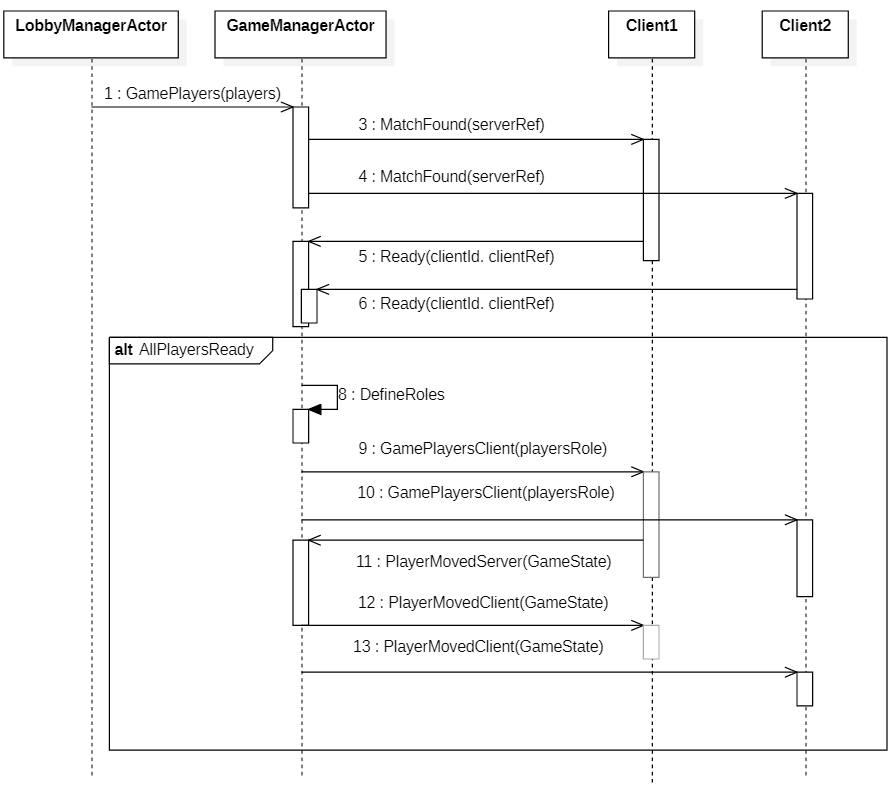
\includegraphics[width=13cm, height=12cm]{doc/report/img/GameServer-Seq-diagram.PNG}
\caption{Sequence Diagram che rappresenta il comportamento del GameManagerActor}
\label{fig:ClasDiagRaprCompGameManagerAct}
\end{figure}

Una volta creato, l'attore responsabile della gestione della partita si occupa, come rappresentato in Figura \ref{fig:ClasDiagRaprCompGameManagerAct}, di:
\begin{itemize}
    \item Rimenere in attesa del messaggio \textit{GamePlayers} di inizializzazione contenente le informazioni dei giocatori;
    \item Notificare i player tramite un messaggio di \textit{MatchFound} che la partita \`e stata trovata;
    \item Rimanere in attesa del messaggio di conferma \textit{Ready} dei Client, avente l'ID del giocatore ed il riferimento dell'attore a cui inviare i messaggi successivi;
    \item Ricevere tutti i messaggi di avvenuta ricezione ed a quel punto inizializzare la partita;
    \item Generare la lista iniziale dei giocatori, scegliendo in base alle impostazioni uno o pi\`u Impostori ed inviandola ai vari Client connessi;
\end{itemize}

Il Client si occupa dell'intercettazione delle azioni eseguite dall'utente durante l'esecuzione del gioco e di comunicarle al Server, ricevendo inoltre le informazioni sullo stato di avanzamento del gioco.\\
Dopo aver inizializzato il gioco, il Server rimane in ascolto di eventuali azioni dei giocatori, che possono essere di due tipi:
\begin{itemize}
    \item Messaggi di aggiornamento dello stato di un giocatore: in questo caso il server va a verificare se vi sono le condizioni di vittoria e notifica la fine della partita, altrimenti ritrasmette l'aggiornamento dello stato a tutti i giocatori;
    \item Messaggio che indica il passaggio alla fase di votazione: in questo caso il Server cambia il suo Comportamento passando dalla fase di gioco alla fase di votazione. In questa fase il Server ha la funzione di raccogliere i voti dai giocatori e di ritrasmettere i vari messaggi inviati tramite la Chat. Una volta raccolti i voti di tutti i giocatori viene selezionato l'eventuale giocatore candidato all'eliminazione se necessario. Viene successivamente controllata se vi \`e una condizione di vittoria, con conseguente notifica di termine partita, altrimenti il gioco torna al comportamento precedente notificando tutti i giocatori;
\end{itemize} 

\newpage
\section{Interazione Attori Client}
Nei diagrammi sottostanti sono rappresentati esempi di come avviene la comunicazione nel dettaglio tra gli attori presenti nel Client.\\
Il flusso di gioco del singolo giocatore viene gestito interamente in locale dal proprio Client.

\begin{figure}[ht]
\centering
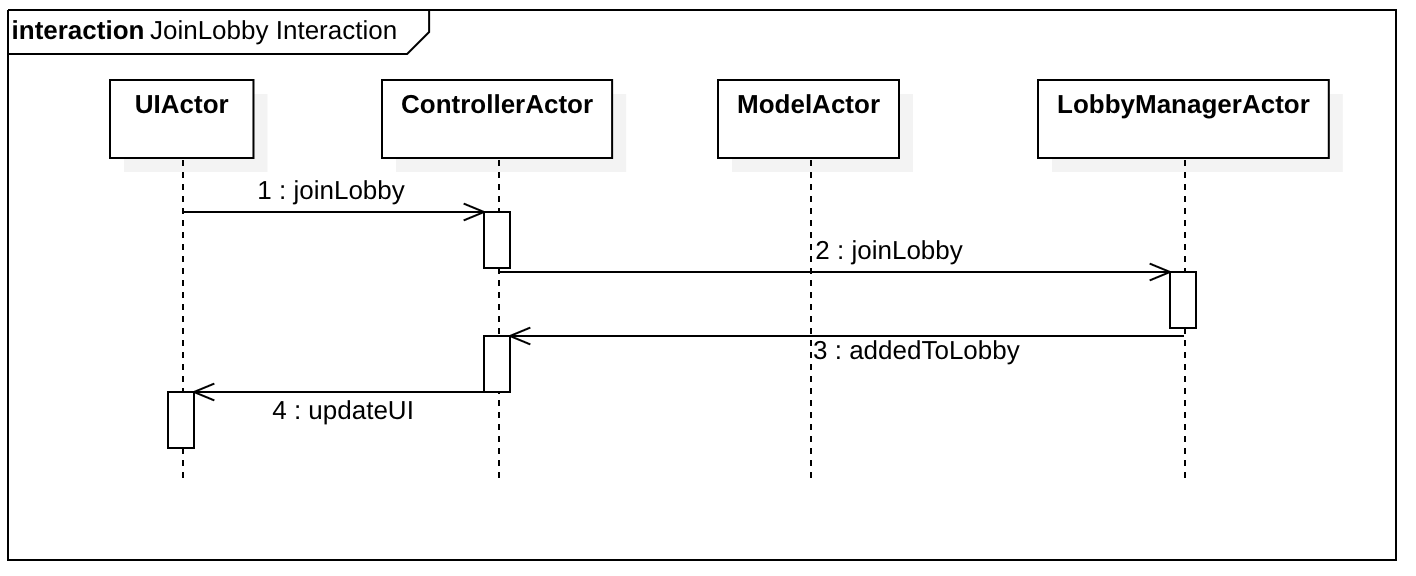
\includegraphics[width=10cm, height=5cm]{img/LobbyInteraction.png}
\caption{Sequence Diagram che rappresenta l'interazione nella fase \textit{Join Lobby}}
\label{fig:ClasDiagRaprInterazJoinToLobby}
\end{figure}

Nella Figura \ref{fig:ClasDiagRaprInterazJoinToLobby} \`e stato rappresentato come avviene l'interazione tra i vari Attori, sia Server che Client, nel momento in cui un player viene aggiunto alla Lobby. In particolare dallo UiActor viene inviato un messaggio di \textit{joinLobby} al \textit{ControllerActor} che notifica al \textit{LobbyManagerActor} il \textit{joinLobby} per aggiungere correttamente il nuovo \textit{Player} alla lobby. Il \textit{ControllerActor} riceve un messaggio di \textit{addedToLobby} del completamento dell'operazione e notifica allo \textit{UiActor} un \textit{updatedUI} che permette l'aggiornamento della \textit{View}.

\begin{figure}[ht]
\centering
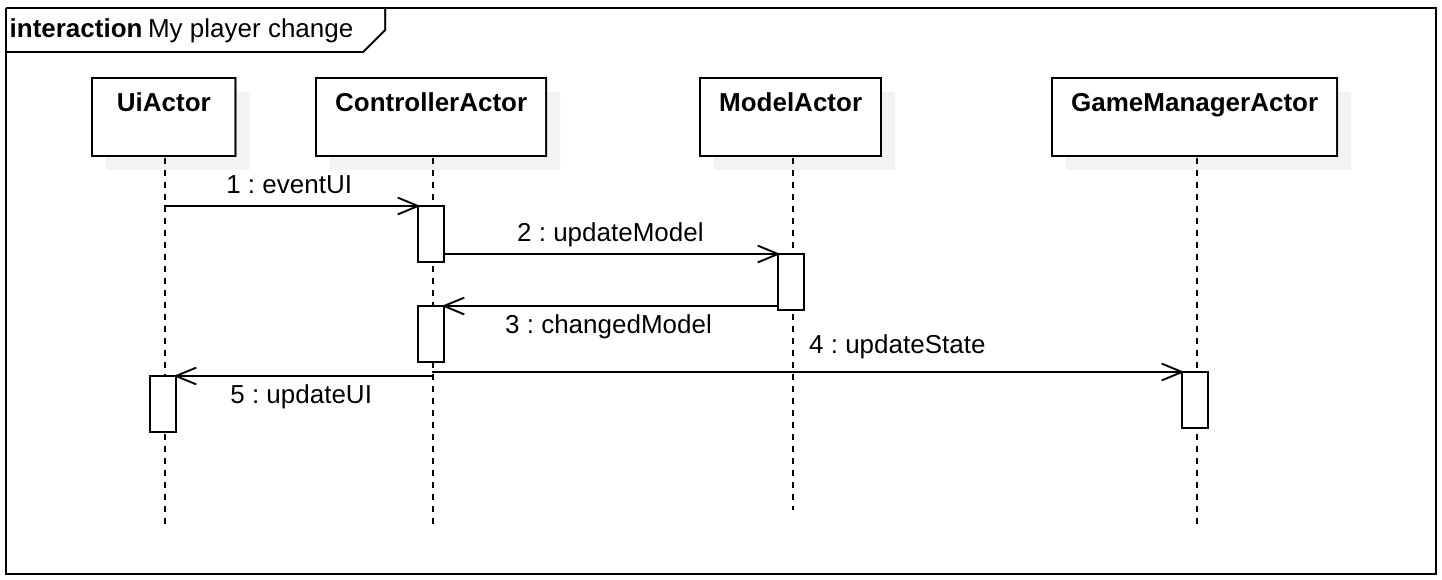
\includegraphics[width=10cm, height=5cm]{img/MyPlayerInteraction.png}
\caption{Sequence Diagram che rappresenta l'interazione a seguito di un azione da parte dell'utente}
\label{fig:ClasDiagRaprInterazDopoAzionUtent}
\end{figure}

La Figura \ref{fig:ClasDiagRaprInterazDopoAzionUtent} rappresenta come il flusso di gioco sia gestito in locale. L'azione dell'utente proveniente dallo \textit{UIActor} viene comunicata al \textit{ControllerActor}. Il \textit{ControllerActor}, dopo aver aggiornato il \textit{ModelActor}, notifica il cambiamento al proprio UiActor. Oltre a questo il \textit{ControllerActor} invia un messaggio anche al GameManagerActor per permettere di aggiornare anche tutti gli altri giocatori connessi. 

\begin{figure}[ht]
\centering
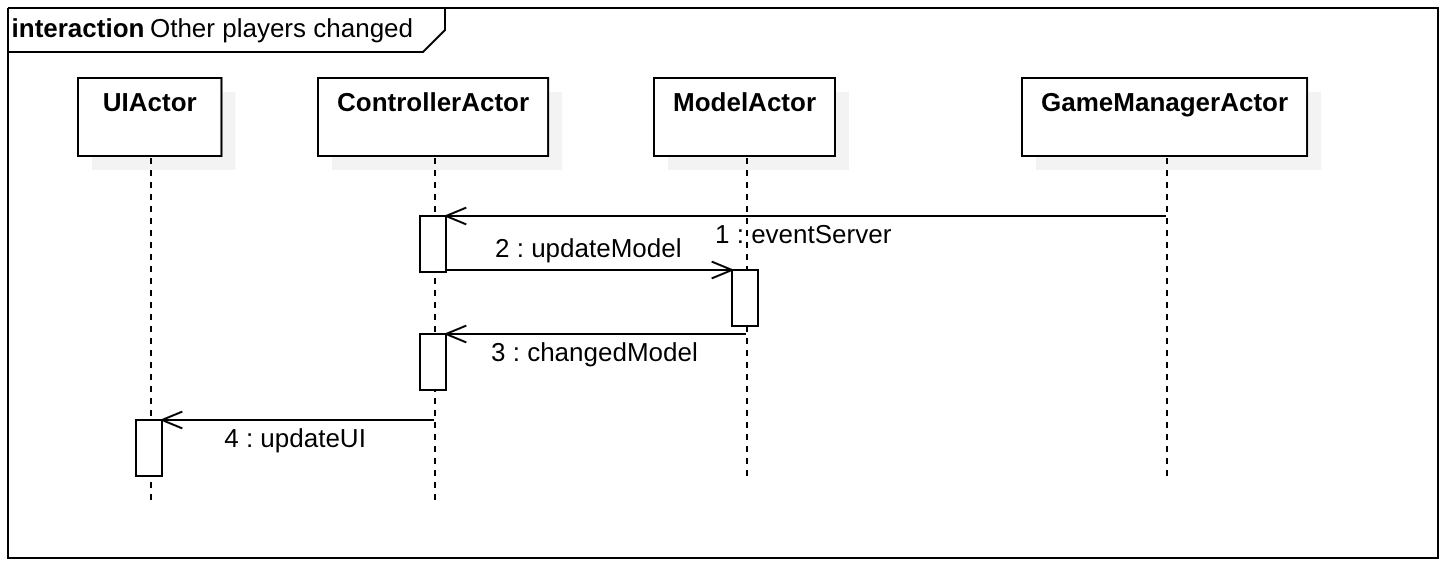
\includegraphics[width=10cm, height=5cm]{img/OtherPlayersInteraction.png}
\caption{Sequence Diagram che rappresenta l'interazione a seguito di un messaggio dal server}
\label{fig:ClasDiagRaprInterazDopoMsgServer}
\end{figure}

Nella Figura \ref{fig:ClasDiagRaprInterazDopoMsgServer} vi è rappresentato il flusso di informazioni generato a seguito di un cambiamento di un altro giocatore.\\
Il messaggio ricevuto dal \textit{ControllerActor} indica che vi è stato un cambiamento di stato da parte di un qualsiasi altro giocatore. Il \textit{ControllerActor} aggiorna lo stato in locale comunicando con il \textit{ModelActor}.\\
Infine aggiorna lo \textit{UiActor} dei cambiamenti effettuati.